	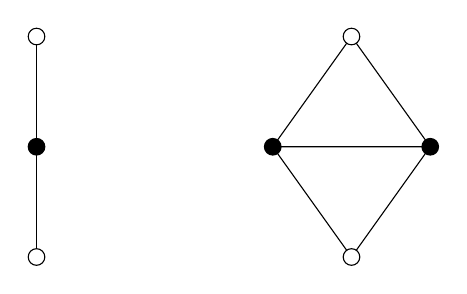
\begin{tikzpicture}
	\def\c{1.4}
	\coordinate (a1) at (1,0);
	\coordinate (a2) at (0,\c);
	\coordinate (a3) at (-1,0);
	\coordinate (a4) at (0,-\c);
	\draw (a1) -- (a2) -- (a3) -- (a4) -- (a1) -- (a3);
	\draw[fill=white] (a2) circle (3pt);
	\draw[fill=white] (a4) circle (3pt);
	\draw[fill=black] (a1) circle (3pt);
	\draw[fill=black] (a3) circle (3pt);
	
	
	\def\a{-4}
	\coordinate (b1) at (\a,-\c);
	\coordinate (b2) at (\a,0);
	\coordinate (b3) at (\a,\c);
	\draw (b1) -- (b2) -- (b3);
	\draw[fill=white] (b1) circle (3pt);
	\draw[fill=white] (b3) circle (3pt);
	\draw[fill=black] (b2) circle (3pt);
	\end{tikzpicture}